\section{Integral triple}

La integral triple acumula los valores de una función $f(x,y,z)$ sobre una región del espacio. A diferencia de una integral doble, la región de integración es un volumen. Si $f$ representa una densidad de masa por unidad de volumen, su integral triple representa la masa total; si $f=1$, representa el volumen del sólido.

Considérese la caja rectangular
\[
B=[a,b]\times[c,d]\times[p,q].
\]
Se divide cada intervalo mediante particiones
\[
a=x_0<\cdots<x_m=b,\qquad c=y_0<\cdots<y_n=d,
\qquad p=z_0<\cdots<z_\ell=q.
\]
Estas particiones producen pequeñas cajas $B_{ijk}$, de volumen
\[
\Delta V_{ijk}=\Delta x_i\,\Delta y_j\,\Delta z_k,
\qquad \Delta x_i=x_i-x_{i-1},
\]
con definiciones análogas para $\Delta y_j$ y $\Delta z_k$. En cada caja se elige un punto
\[
P_{ijk}^*=(x_{ijk}^*,y_{ijk}^*,z_{ijk}^*).
\]
El producto $f(P_{ijk}^*)\Delta V_{ijk}$ aproxima la contribución de esa caja y la suma triple
\[
S=\sum_{i=1}^{m}\sum_{j=1}^{n}\sum_{k=1}^{\ell}
f(P_{ijk}^*)\,\Delta V_{ijk}
\]
acumula las contribuciones de todas ellas. Los tres índices recorren las subdivisiones en las direcciones $x$, $y$ y $z$.

\begingroup
\shorthandoff{>}
\begin{center}
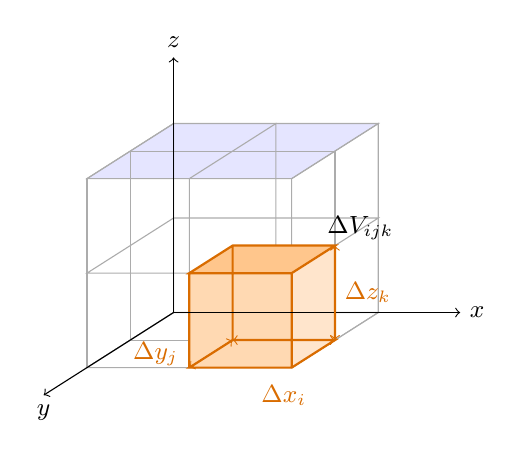
\begin{tikzpicture}[x={(2.6cm,0cm)},y={(-1.1cm,-0.7cm)},z={(0cm,2.4cm)},every node/.style={font=\small}]
    \fill[blue!10] (0,0,1) -- (1,0,1) -- (1,1,1) -- (0,1,1) -- cycle;
    \foreach \t in {0,.5,1} {
        \draw[gray!65] (\t,0,0) -- (\t,1,0) -- (\t,1,1) -- (\t,0,1) -- cycle;
        \draw[gray!65] (0,\t,0) -- (1,\t,0) -- (1,\t,1) -- (0,\t,1) -- cycle;
        \draw[gray!65] (0,0,\t) -- (1,0,\t) -- (1,1,\t) -- (0,1,\t) -- cycle;
    }
    % Las tres caras visibles de la subcaja B_{ijk}.
    \fill[orange!45] (.5,.5,.5) -- (1,.5,.5) -- (1,1,.5) -- (.5,1,.5) -- cycle;
    \fill[orange!30] (.5,1,0) -- (1,1,0) -- (1,1,.5) -- (.5,1,.5) -- cycle;
    \fill[orange!20] (1,.5,0) -- (1,1,0) -- (1,1,.5) -- (1,.5,.5) -- cycle;
    \draw[orange!85!black,thick]
        (.5,.5,0) -- (1,.5,0) -- (1,1,0) -- (.5,1,0) -- cycle
        (.5,.5,.5) -- (1,.5,.5) -- (1,1,.5) -- (.5,1,.5) -- cycle
        (.5,.5,0) -- (.5,.5,.5)
        (1,.5,0) -- (1,.5,.5)
        (1,1,0) -- (1,1,.5)
        (.5,1,0) -- (.5,1,.5);
    \draw[->] (0,0,0) -- (1.4,0,0) node[right] {$x$};
    \draw[->] (0,0,0) -- (0,1.5,0) node[below] {$y$};
    \draw[->] (0,0,0) -- (0,0,1.35) node[above] {$z$};
    \draw[<->,orange!85!black] (.5,.5,0) -- (1,.5,0)
        node[midway, yshift=-20pt] {$\Delta x_i$};
    \draw[<->,orange!85!black] (.5,.5,0) -- (.5,1,0)
        node[midway, xshift=-20pt] {$\Delta y_j$};
    \draw[<->,orange!85!black] (1,.5,0) -- (1,.5,.5)
        node[midway,right] {$\Delta z_k$};
    \node[right] at (1,.7,.65) {$\Delta V_{ijk}$};
\end{tikzpicture}
\end{center}
\endgroup

La figura representa una partición de una caja en ocho subcajas; la subcaja resaltada tiene volumen igual al producto de sus tres longitudes.

Por analogía de la integral doble, se define la integral triple como el límite de las sumas de Riemann sobre las subcajas de una partición de la caja.

\begin{mydefinition}{Integral triple sobre una caja}
Sea $f:B\to\mathbb{R}$ una función acotada en una caja rectangular cerrada $B$. La integral triple de $f$ sobre $B$ se define como:
\[
\iiint_B f(x,y,z)\,dV
=\lim_{\ell, m, n \to \infty}
\sum_{i=1}^{m}\sum_{j=1}^{n}\sum_{k=1}^{\ell}
f(P_{ijk}^*)\,\Delta x_i\,\Delta y_j\,\Delta z_k
\]
Toda función continua en $B$ es integrable. El símbolo $dV$ representa un elemento de volumen.
\end{mydefinition}

La integral triple siempre existe si la función es continua.

Por otro lado, al igual que en las integrales dobles, es posible cambiar el orden de integración en las integrales triples, siempre y cuando la función sea continua.

\subsection{Teorema de Fubini para integrales triples}

\begin{mytheorem}{Fubini en una caja rectangular}
Si $f$ es continua en $B=[a,b]\times[c,d]\times[p,q]$, entonces su integral triple puede calcularse mediante integrales iteradas en cualquiera de los seis órdenes:
\begin{align*}
\iiint_B f\,dV
&=\int_a^b\int_c^d\int_p^q f(x,y,z)\,dz\,dy\,dx
=\int_a^b\int_p^q\int_c^d f(x,y,z)\,dy\,dz\,dx\\
&=\int_c^d\int_a^b\int_p^q f(x,y,z)\,dz\,dx\,dy
=\int_c^d\int_p^q\int_a^b f(x,y,z)\,dx\,dz\,dy\\
&=\int_p^q\int_a^b\int_c^d f(x,y,z)\,dy\,dx\,dz
=\int_p^q\int_c^d\int_a^b f(x,y,z)\,dx\,dy\,dz.
\end{align*}
\end{mytheorem}

Las integrales se calculan desde la más interior hacia la más exterior. En el orden $dz\,dy\,dx$ se integra primero respecto de $z$, manteniendo $x$ e $y$ constantes; el resultado depende de $x$ e $y$. Después se integra respecto de $y$, con $x$ constante, y finalmente respecto de $x$.

\subsubsection*{Ejemplo: integral de una función en una caja}

Para $f(x,y,z)=x+2y+3z$ y $B=[0,1]\times[0,2]\times[0,1]$, se tiene
\begin{align*}
\iiint_B f\,dV
&=\int_0^1\int_0^2\int_0^1(x+2y+3z)\,dz\,dy\,dx\\
&=\int_0^1\int_0^2\left[xz+2yz+\frac32z^2\right]_{z=0}^{z=1}\,dy\,dx\\
&=\int_0^1\int_0^2\left(x+2y+\frac32\right)\,dy\,dx
=\int_0^1(2x+7)\,dx=8.
\end{align*}
La caja tiene volumen $2$, pero esta integral vale $8$ porque el integrando no es $1$. En particular, la integral triple de una función positiva no representa, en general, el volumen de la región sobre la que se integra.

\subsection{La integral triple sobre una región general}

\begin{mydefinition}{Integral triple sobre un sólido acotado}
Sea $E\subset\mathbb R^3$ un sólido acotado, contenido en una caja $B$, y sea $f:E\to\mathbb R$ acotada. Se extiende $f$ a $B$ por
\[
\widetilde f(x,y,z)=
\begin{cases}
f(x,y,z),&(x,y,z)\in E,\\
0,&(x,y,z)\in B\setminus E.
\end{cases}
\]
Si $\widetilde f$ es integrable en $B$, se define
\[
\iiint_E f\,dV=\iiint_B\widetilde f\,dV.
\]
La definición no depende de la caja que contiene a $E$.
\end{mydefinition}

En este tema se consideran sólidos cerrados y acotados con fronteras formadas por un número finito de superficies suaves por partes, y funciones continuas sobre ellos. Estas condiciones garantizan la integrabilidad: las cajas que cortan la frontera pueden cubrirse con volumen total tan pequeño como se desee. La extensión por cero puede ser discontinua en la frontera, pero esas discontinuidades no impiden que exista la integral.

Se conservan la linealidad y la aditividad respecto de la región. Si $E$ se divide en sólidos $E_1$ y $E_2$ cuyos interiores no se superponen y que solo comparten superficies de frontera, entonces
\[
\iiint_E f\,dV=\iiint_{E_1}f\,dV+\iiint_{E_2}f\,dV.
\]

Para poder definir la integral triple sobre un sólido general, es útil considerar sólidos que sean simples en alguna dirección, de manera que los límites de integración puedan expresarse de forma explícita.

Un sólido es simple en la dirección $z$ si, al fijar $(x,y)$ en su proyección $D_{xy}$, los valores admisibles de $z$ forman un solo intervalo:
\[
E=\{(x,y,z):(x,y)\in D_{xy},\ u(x,y)\leq z\leq v(x,y)\}.
\]
La proyección $D_{xy}$ contiene exactamente los puntos $(x,y)$ para los cuales existe al menos un $z$ con $(x,y,z)\in E$. Geométricamente, se sigue una recta paralela al eje $z$: $u$ es la superficie de entrada y $v$ la de salida. No se requiere que ambas alturas sean positivas, sino que $u\leq v$ en la proyección.

\begingroup
\shorthandoff{>}
\begin{center}
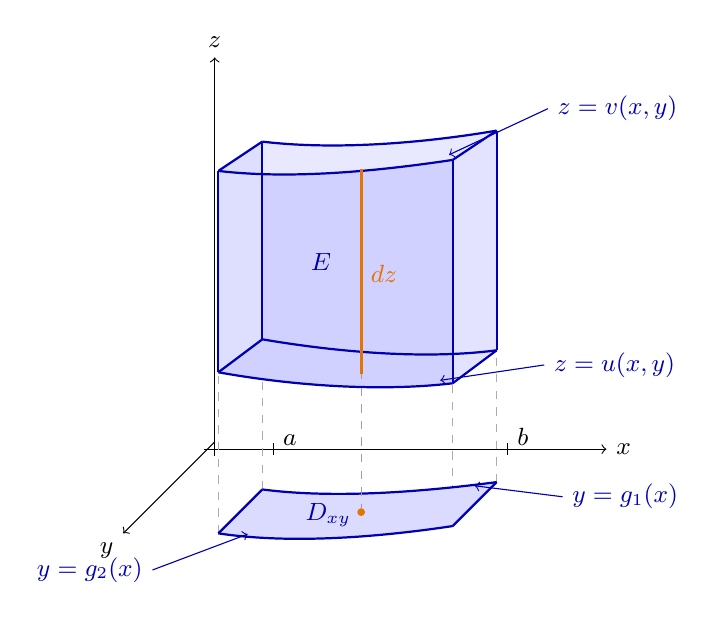
\begin{tikzpicture}[scale=.93, every node/.style={font=\small}]
    % Ejes coordenados.
    \draw[->] (-.15,0) -- (5.35,0) node[right] {$x$};
    \draw[->] (0,.1) -- (-1.25,-1.15) node[below left] {$y$};
    \draw[->] (0,-.1) -- (0,5.35) node[above] {$z$};
    \draw (.8,.08) -- (.8,-.08) node[above right] {$a$};
    \draw (4,.08) -- (4,-.08) node[above right] {$b$};

    % Líneas que muestran la proyección del sólido sobre el plano xy.
    \draw[dashed,gray!65] (.05,-1.15) -- (.05,1.05);
    \draw[dashed,gray!65] (.65,-.55) -- (.65,1.5);
    \draw[dashed,gray!65] (3.25,-1.05) -- (3.25,.9);
    \draw[dashed,gray!65] (3.85,-.45) -- (3.85,1.35);

    % Región plana D_{xy}.
    \fill[blue!14]
        (.65,-.55) .. controls (1.65,-.68) and (2.85,-.58) .. (3.85,-.45)
        -- (3.25,-1.05)
        .. controls (2.25,-1.2) and (1.05,-1.3) .. (.05,-1.15) -- cycle;
    \draw[blue!70!black,thick]
        (.65,-.55) .. controls (1.65,-.68) and (2.85,-.58) .. (3.85,-.45);
    \draw[blue!70!black,thick]
        (.05,-1.15) .. controls (1.05,-1.3) and (2.25,-1.2) .. (3.25,-1.05);
    \draw[blue!70!black,thick] (.65,-.55) -- (.05,-1.15);
    \draw[blue!70!black,thick] (3.85,-.45) -- (3.25,-1.05);

    % Sólido comprendido entre z=u(x,y) y z=v(x,y).
    \fill[blue!18]
        (.05,1.05) .. controls (1.05,.87) and (2.25,.78) .. (3.25,.9)
        -- (3.25,3.95)
        .. controls (2.25,3.8) and (1.05,3.68) .. (.05,3.8) -- cycle;
    \fill[blue!11]
        (3.25,.9) -- (3.85,1.35) -- (3.85,4.35) -- (3.25,3.95) -- cycle;
    \fill[blue!9]
        (.05,3.8) .. controls (1.05,3.68) and (2.25,3.8) .. (3.25,3.95)
        -- (3.85,4.35)
        .. controls (2.85,4.18) and (1.65,4.08) .. (.65,4.2) -- cycle;
    \fill[blue!13]
        (.05,1.05) -- (.65,1.5) -- (.65,4.2) -- (.05,3.8) -- cycle;

    \draw[blue!70!black,thick]
        (.05,1.05) .. controls (1.05,.87) and (2.25,.78) .. (3.25,.9);
    \draw[blue!70!black,thick]
        (.65,1.5) .. controls (1.65,1.33) and (2.85,1.22) .. (3.85,1.35);
    \draw[blue!70!black,thick]
        (.05,3.8) .. controls (1.05,3.68) and (2.25,3.8) .. (3.25,3.95);
    \draw[blue!70!black,thick]
        (.65,4.2) .. controls (1.65,4.08) and (2.85,4.18) .. (3.85,4.35);
    \draw[blue!70!black,thick]
        (.05,1.05) -- (.05,3.8)
        (.65,1.5) -- (.65,4.2)
        (3.25,.9) -- (3.25,3.95)
        (3.85,1.35) -- (3.85,4.35);
    \draw[blue!70!black,thick] (.05,1.05) -- (.65,1.5);
    \draw[blue!70!black,thick] (3.25,.9) -- (3.85,1.35);
    \draw[blue!70!black,thick] (.05,3.8) -- (.65,4.2);
    \draw[blue!70!black,thick] (3.25,3.95) -- (3.85,4.35);

    % Segmento vertical correspondiente a un punto de D_{xy}.
    \draw[dashed,gray!75] (2,-.86) -- (2,1.02);
    \fill[orange!90!black] (2,-.86) circle (1.5pt);
    \draw[orange!90!black,very thick] (2,1.02) -- (2,3.83);
    \node[orange!90!black,right] at (2,2.4) {$dz$};

    % Etiquetas, colocadas fuera de las fronteras para mantener legibilidad.
    \node[blue!70!black] at (1.55,-.9) {$D_{xy}$};
    \node[blue!70!black] at (1.45,2.55) {$E$};
    \draw[->,blue!70!black] (4.55,4.65) node[right] {$z=v(x,y)$} -- (3.2,4.02);
    \draw[->,blue!70!black] (4.5,1.15) node[right] {$z=u(x,y)$} -- (3.08,.94);
    \draw[->,blue!70!black] (4.75,-.65) node[right] {$y=g_1(x)$} -- (3.55,-.5);
    \draw[->,blue!70!black] (-.85,-1.65) node[left] {$y=g_2(x)$} -- (.45,-1.16);
\end{tikzpicture}
\end{center}
\endgroup

La recta naranja representa el segmento de integración asociado con un punto de $D_{xy}$. Al recorrer todos los puntos de la proyección, esos segmentos llenan el sólido $E$.

\begin{mytheorem}{Integración sobre un sólido simple}
Sea $D_{xy}$ una región plana cerrada y acotada con frontera suave por partes, y sean $u,v$ continuas en $D_{xy}$, con $u\leq v$. Si $f$ es continua en el sólido $E$ entonces
\[
\iiint_E f(x,y,z)\,dV
=\iint_{D_{xy}}\left(\int_{u(x,y)}^{v(x,y)}f(x,y,z)\,dz\right)dA.
\]
En particular, si $D_{xy}=\{(x,y):a\leq x\leq b,\ g_1(x)\leq y\leq g_2(x)\}$, con fronteras continuas, se obtiene
\[
\iiint_E f\,dV
=\int_a^b\int_{g_1(x)}^{g_2(x)}\int_{u(x,y)}^{v(x,y)}
f(x,y,z)\,dz\,dy\,dx.
\]
\end{mytheorem}

Este teorema puede aplicarse a regiones E que son simples con respecto a cualquiera de los ejes coordenados, siendo necesario hacer los ajustes correspondientes en los límites de integración y el orden de los diferenciales.

\subsubsection{Las otras direcciones y los seis órdenes}

Si se integra primero respecto de $y$, se proyecta sobre $xz$; si se integra primero respecto de $x$, se proyecta sobre $yz$. Por ejemplo,
\begin{align*}
E&=\{(x,y,z):a\leq x\leq b,\ r_1(x)\leq z\leq r_2(x),\
s_1(x,z)\leq y\leq s_2(x,z)\},\\
\iiint_E f\,dV
&=\int_a^b\int_{r_1(x)}^{r_2(x)}\int_{s_1(x,z)}^{s_2(x,z)}
f(x,y,z)\,dy\,dz\,dx.
\end{align*}

\paragraph{Ejemplo 1. Un tetraedro} Sea
\[
E=\{(x,y,z):x\geq0,\ y\geq0,\ z\geq0,\ x+y+z\leq1\}.
\]
Para integrar primero en $z$, se fijan $x,y$ y se obtiene $0\leq z\leq1-x-y$. El intervalo existe si $x+y\leq1$. Por tanto,
\[
D_{xy}=\{(x,y):0\leq x\leq1,\ 0\leq y\leq1-x\}.
\]

\begingroup
\shorthandoff{>}
\begin{center}
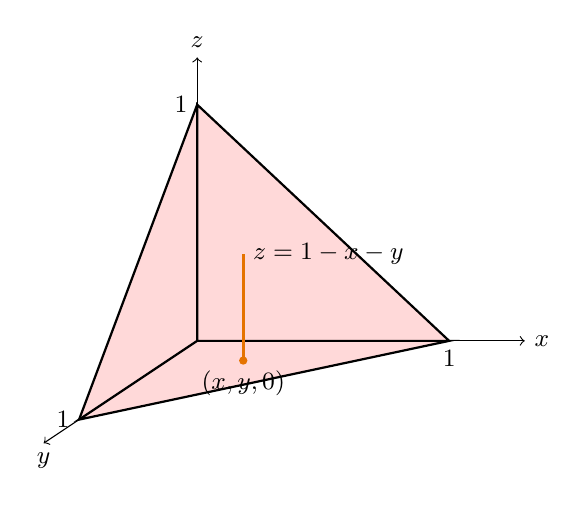
\begin{tikzpicture}[x={(3.2cm,0cm)},y={(-1.5cm,-1cm)},z={(0cm,3cm)},every node/.style={font=\small}]
    \fill[blue!18] (0,0,0) -- (1,0,0) -- (0,1,0) -- cycle;
    \fill[red!15] (1,0,0) -- (0,1,0) -- (0,0,1) -- cycle;
    \draw[thick] (0,0,0) -- (1,0,0) -- (0,1,0) -- (0,0,0) -- (0,0,1) -- (1,0,0);
    \draw[thick] (0,1,0) -- (0,0,1);
    \draw[->] (0,0,0) -- (1.3,0,0) node[right] {$x$};
    \draw[->] (0,0,0) -- (0,1.3,0) node[below] {$y$};
    \draw[->] (0,0,0) -- (0,0,1.2) node[above] {$z$};
    \draw[orange!90!black,very thick] (.3,.25,0) -- (.3,.25,.45);
    \fill[orange!90!black] (.3,.25,0) circle (1.5pt);
    \node[right] at (.3,.25,.45) {$z=1-x-y$};
    \node[below] at (.3,.25,0) {$(x,y,0)$};
    \node[below] at (1,0,0) {$1$};
    \node[left] at (0,1,0) {$1$};
    \node[left] at (0,0,1) {$1$};
\end{tikzpicture}
\hspace{.5cm}
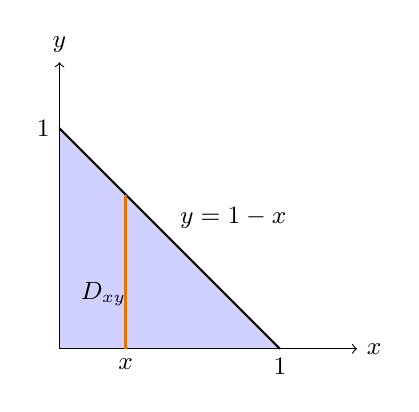
\begin{tikzpicture}[scale=2.8,every node/.style={font=\small}]
    \fill[blue!18] (0,0) -- (1,0) -- (0,1) -- cycle;
    \draw[->] (0,0) -- (1.35,0) node[right] {$x$};
    \draw[->] (0,0) -- (0,1.3) node[above] {$y$};
    \draw[thick] (0,1) -- (1,0) node[midway,above right] {$y=1-x$};
    \draw[orange!90!black,very thick] (.3,0) -- (.3,.7);
    \node[below] at (.3,0) {$x$};
    \node[below] at (1,0) {$1$};
    \node[left] at (0,1) {$1$};
    \node at (.2,.25) {$D_{xy}$};
\end{tikzpicture}
\end{center}
\endgroup

El segmento naranja del sólido da los límites de $z$. El segmento naranja de la proyección da los límites de $y$ cuando $x$ queda fijo. Por ello,
\begin{align*}
V(E)&=\int_0^1\int_0^{1-x}\int_0^{1-x-y}1\,dz\,dy\,dx\\
&=\int_0^1\int_0^{1-x}(1-x-y)\,dy\,dx
=\frac12\int_0^1(1-x)^2\,dx=\frac16.
\end{align*}
La simetría de las desigualdades permite escribir los seis órdenes sin dividir la región. Para cualquier $f$ continua en $E$, se tiene
\begin{align*}
\iiint_E f\,dV
&=\int_0^1\int_0^{1-x}\int_0^{1-x-y}f(x,y,z)\,dz\,dy\,dx\\
&=\int_0^1\int_0^{1-y}\int_0^{1-x-y}f(x,y,z)\,dz\,dx\,dy\\
&=\int_0^1\int_0^{1-x}\int_0^{1-x-z}f(x,y,z)\,dy\,dz\,dx\\
&=\int_0^1\int_0^{1-z}\int_0^{1-x-z}f(x,y,z)\,dy\,dx\,dz\\
&=\int_0^1\int_0^{1-y}\int_0^{1-y-z}f(x,y,z)\,dx\,dz\,dy\\
&=\int_0^1\int_0^{1-z}\int_0^{1-y-z}f(x,y,z)\,dx\,dy\,dz.
\end{align*}
En cada renglón la variable interior queda acotada por $1$ menos las otras dos; la intermedia queda acotada por $1$ menos la exterior.

\paragraph{Ejemplo 2. Entre un paraboloide y un plano}

El sólido encerrado entre $z=x^2+y^2$ y $z=1$ satisface
\[
x^2+y^2\leq z\leq1.
\]
Las superficies se intersectan cuando $x^2+y^2=1$. La condición para que exista el segmento vertical es $x^2+y^2\leq1$, de modo que la proyección es el disco unitario, aunque el sólido solo toca el plano $xy$ en el origen. En coordenadas cartesianas,
\[
V=\int_{-1}^1\int_{-\sqrt{1-x^2}}^{\sqrt{1-x^2}}
\int_{x^2+y^2}^{1}1\,dz\,dy\,dx.
\]

\begingroup
\shorthandoff{>}
\begin{center}
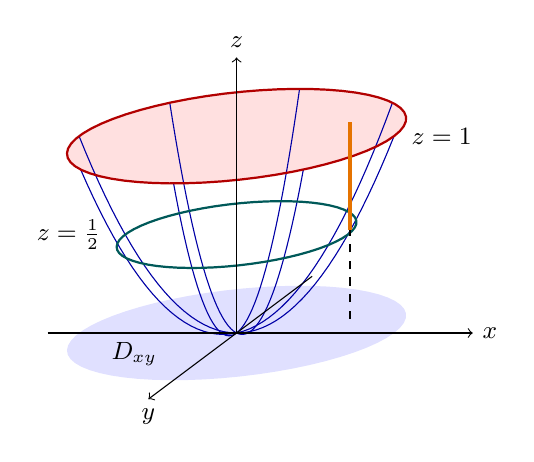
\begin{tikzpicture}[x={(2cm,0cm)},y={(-.8cm,-.6cm)},z={(0cm,2.5cm)},every node/.style={font=\small}]
    \fill[blue!12] plot[domain=0:360,samples=60] ({cos(\x)},{sin(\x)},0) -- cycle;
    \fill[red!12] plot[domain=0:360,samples=60] ({cos(\x)},{sin(\x)},1) -- cycle;
    \foreach \ang in {0,45,...,315} {
        \draw[blue!65!black] plot[domain=0:1,samples=25] ({\x*cos(\ang)},{\x*sin(\ang)},{\x*\x});
    }
    \draw[red!70!black,thick] plot[domain=0:360,samples=60] ({cos(\x)},{sin(\x)},1);
    \draw[teal!70!black,thick] plot[domain=0:360,samples=60] ({.7071*cos(\x)},{.7071*sin(\x)},.5);
    \draw[orange!90!black,very thick] (.6,-.3,.45) -- (.6,-.3,1);
    \draw[dashed] (.6,-.3,0) -- (.6,-.3,.45);
    \draw[->] (-1.2,0,0) -- (1.5,0,0) node[right] {$x$};
    \draw[->] (0,-1.2,0) -- (0,1.4,0) node[below] {$y$};
    \draw[->] (0,0,0) -- (0,0,1.4) node[above] {$z$};
    \node[right] at (1.05,0,1) {$z=1$};
    \node[left] at (-.8,0,.5) {$z=\frac12$};
    \node[below] at (-.65,0,0) {$D_{xy}$};
\end{tikzpicture}
\hspace{.5cm}
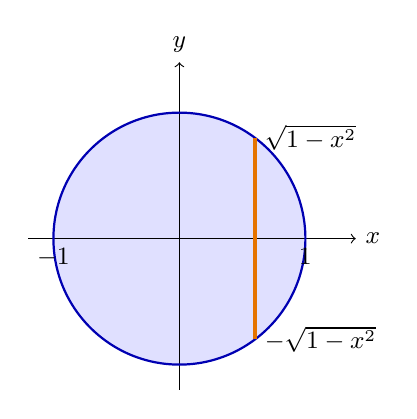
\begin{tikzpicture}[scale=1.6,every node/.style={font=\small}]
    \fill[blue!12] (0,0) circle (1);
    \draw[->] (-1.2,0) -- (1.4,0) node[right] {$x$};
    \draw[->] (0,-1.2) -- (0,1.4) node[above] {$y$};
    \draw[blue!70!black,thick] (0,0) circle (1);
    \draw[orange!90!black,very thick] (.6,-.8) -- (.6,.8);
    \node[right] at (.6,.8) {$\sqrt{1-x^2}$};
    \node[right] at (.6,-.8) {$-\sqrt{1-x^2}$};
    \node[below] at (-1,0) {$-1$};
    \node[below] at (1,0) {$1$};
\end{tikzpicture}
\end{center}
\endgroup

La curva verde representa la frontera del corte horizontal $z=1/2$. En general, a altura fija $z$, el corte es $x^2+y^2\leq z$, un disco de radio $\sqrt z$; las alturas recorren $0\leq z\leq1$. Esto proporciona otro orden:
\[
V=\int_0^1\int_{-\sqrt z}^{\sqrt z}
\int_{-\sqrt{z-x^2}}^{\sqrt{z-x^2}}1\,dy\,dx\,dz.
\]
La integral doble interior es el área del disco de radio $\sqrt z$, es decir, $\pi z$. Por tanto,
\[
V=\int_0^1\pi z\,dz=\frac\pi2.
\]
La elección de $z$ como variable exterior permite usar directamente el área de los cortes. Las raíces se toman con ambos signos porque los discos incluyen coordenadas positivas y negativas.

\paragraph{Ejemplo 3. Integración primero en \texorpdfstring{$y$}{y}}

Sea $E$ la región descrita por
\[
0\leq x\leq1,\qquad x^2\leq y\leq1,\qquad 0\leq z\leq y.
\]
La superficie $y=x^2$ es un cilindro parabólico paralelo al eje $z$. En el orden dado se tendría $dz\,dy\,dx$. Para integrar primero en $y$, sus restricciones se reúnen como
\[
\max\{x^2,z\}\leq y\leq1.
\]

\begin{samepage}
\begingroup
\shorthandoff{>}
\begin{center}
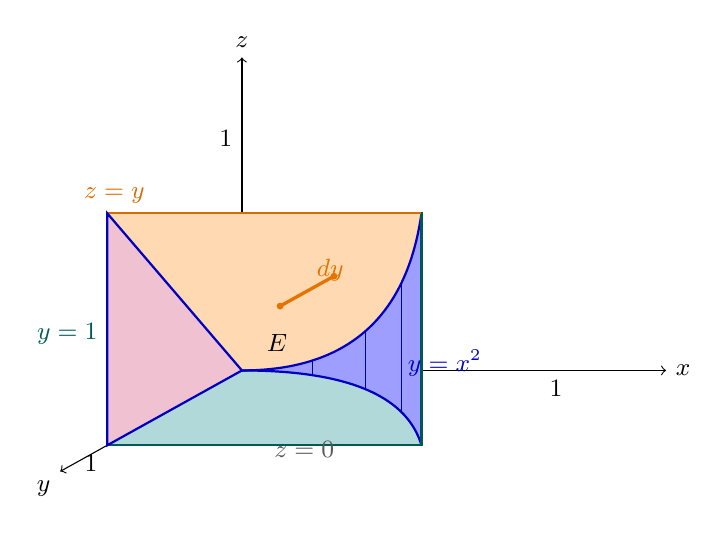
\begin{tikzpicture}[
    x={(4.2cm,0cm)}, y={(-1.8cm,-1cm)}, z={(0cm,3.1cm)},
    scale=.95, every node/.style={font=\small}]
    % Ejes coordenados.
    \draw[->] (0,0,0) -- (1.35,0,0) node[right] {$x$};
    \draw[->] (0,0,0) -- (0,1.35,0) node[below left] {$y$};
    \draw[->] (0,0,0) -- (0,0,1.35) node[above] {$z$};

    % Base z=0, comprendida entre y=x^2 y y=1.
    \fill[gray!18]
        plot[domain=0:1,samples=45] (\x,{\x*\x},0)
        -- plot[domain=1:0,samples=2] (\x,1,0) -- cycle;

    % Cara vertical y=1 y cara triangular x=0.
    \fill[teal!30] (0,1,0) -- (1,1,0) -- (1,1,1) -- (0,1,1) -- cycle;
    \fill[purple!24] (0,0,0) -- (0,1,0) -- (0,1,1) -- cycle;

    % Cilindro parabólico y=x^2, desde z=0 hasta z=y.
    \fill[blue!38]
        plot[domain=0:1,samples=45] (\x,{\x*\x},0)
        -- plot[domain=1:0,samples=45] (\x,{\x*\x},{\x*\x}) -- cycle;

    % Techo inclinado z=y.
    \fill[orange!30]
        plot[domain=0:1,samples=45] (\x,{\x*\x},{\x*\x})
        -- plot[domain=1:0,samples=2] (\x,1,1) -- cycle;

    % Fronteras de las cuatro superficies principales.
    \draw[blue!75!black,thick]
        plot[domain=0:1,samples=45] (\x,{\x*\x},0);
    \draw[blue!75!black,thick]
        plot[domain=0:1,samples=45] (\x,{\x*\x},{\x*\x});
    \draw[teal!70!black,thick] (0,1,0) -- (1,1,0) -- (1,1,1) -- (0,1,1) -- cycle;
    \draw[orange!85!black,thick] (0,1,1) -- (1,1,1);
    \draw[blue!75!black,thick] (0,0,0) -- (0,1,0) -- (0,1,1) -- cycle;
    \foreach \t in {.25,.5,.75} {
        \draw[blue!65!black] (\t,{\t*\t},0) -- (\t,{\t*\t},{\t*\t});
    }

    % Segmento paralelo al eje y para el orden dy dz dx.
    \draw[orange!90!black,very thick] (.55,.6,.6) -- (.55,1,.6);
    \fill[orange!90!black] (.55,.6,.6) circle (1.3pt);
    \fill[orange!90!black] (.55,1,.6) circle (1.3pt);
    \node[orange!90!black,above right] at (.55,.8,.6) {$dy$};

    % Etiquetas.
    \node at (.42,.72,.35) {$E$};
    \node[orange!85!black,above left] at (.15,1,1) {$z=y$};
    \node[teal!70!black,left] at (0,1,.48) {$y=1$};
    \node[blue!75!black,right] at (.72,.52,.2) {$y=x^2$};
    \node[gray!70!black,below] at (.55,.82,0) {$z=0$};
    \node[below] at (1,0,0) {$1$};
    \node[below left] at (0,1,0) {$1$};
    \node[left] at (0,0,1) {$1$};
\end{tikzpicture}
\end{center}
\endgroup

La cara inferior marcada por $z=0$ es la región $x^2\leq y\leq1$ del plano $xy$. Sobre cada punto de esta base, el sólido se extiende hasta el plano $z=y$. El segmento naranja muestra un intervalo paralelo al eje $y$, cuyo extremo inicial está determinado por $\max\{x^2,z\}$ y cuyo extremo final se encuentra en $y=1$.
\end{samepage}

La proyección sobre $xz$ es el cuadrado $0\leq x\leq1$, $0\leq z\leq1$, pero la superficie de entrada cambia en $z=x^2$. Por ello,
\begin{align*}
\iiint_E f\,dV
&=\int_0^1\int_0^{x^2}\int_{x^2}^1 f(x,y,z)\,dy\,dz\,dx\\
&\quad+\int_0^1\int_{x^2}^1\int_z^1 f(x,y,z)\,dy\,dz\,dx.
\end{align*}

\begingroup
\shorthandoff{>}
\begin{center}
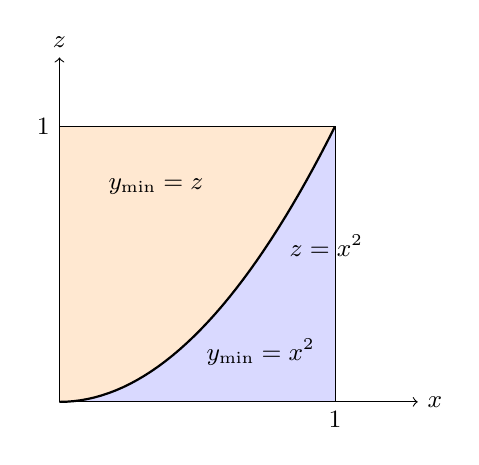
\begin{tikzpicture}[scale=3.5,every node/.style={font=\small}]
    \fill[blue!15] (0,0) -- plot[domain=0:1,samples=40] (\x,{\x*\x}) -- (1,0) -- cycle;
    \fill[orange!18] plot[domain=0:1,samples=40] (\x,{\x*\x}) -- (1,1) -- (0,1) -- cycle;
    \draw[->] (0,0) -- (1.3,0) node[right] {$x$};
    \draw[->] (0,0) -- (0,1.25) node[above] {$z$};
    \draw (0,1) -- (1,1) -- (1,0);
    \draw[thick] plot[domain=0:1,samples=40] (\x,{\x*\x});
    \node[below right] at (.8,.64) {$z=x^2$};
    \node at (.73,.18) {$y_{\min}=x^2$};
    \node at (.35,.78) {$y_{\min}=z$};
    \node[below] at (1,0) {$1$};
    \node[left] at (0,1) {$1$};
\end{tikzpicture}
\end{center}
\endgroup

Para el volumen, integrar primero en $z$ requiere menos partes:
\begin{align*}
V&=\int_0^1\int_{x^2}^1\int_0^y1\,dz\,dy\,dx
=\int_0^1\int_{x^2}^1 y\,dy\,dx\\
&=\frac12\int_0^1(1-x^4)\,dx=\frac25.
\end{align*}
También se puede evitar la división integrando primero en $x$: las desigualdades equivalen a $0\leq y\leq1$, $0\leq z\leq y$ y $0\leq x\leq\sqrt y$. Entonces
\[
V=\int_0^1\int_0^y\int_0^{\sqrt y}1\,dx\,dz\,dy
=\int_0^1 y\sqrt y\,dy=\frac25.
\]

\paragraph{Ejemplo 4. Integración primero en \texorpdfstring{$x$}{x}}

Se considera el sólido
\[
E=\{(x,y,z):0\leq y\leq1,\ 0\leq z\leq1-y,\ y+z\leq x\leq2\}
\]
con densidad $\rho(x,y,z)=x$. Para cada $(y,z)$ del triángulo $D_{yz}$, el segmento paralelo al eje $x$ comienza en el plano $x=y+z$ y termina en $x=2$. La densidad es no negativa en el sólido.

\begingroup
\shorthandoff{>}
\begin{center}
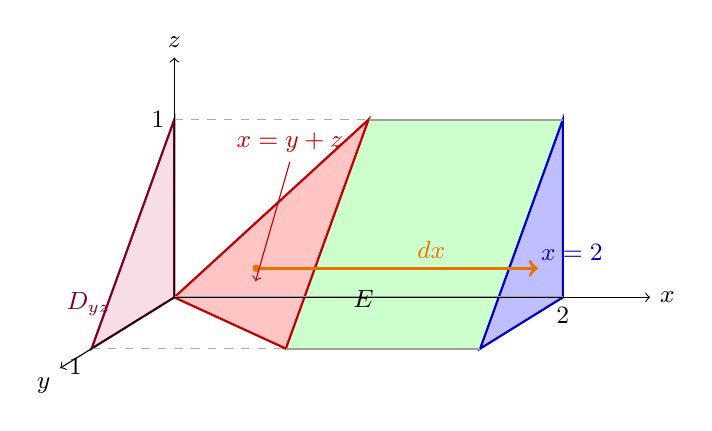
\begin{tikzpicture}[
    x={(2.35cm,0cm)}, y={(-1cm,-.62cm)}, z={(0cm,2.15cm)},
    scale=1.05, every node/.style={font=\small}]
    % Proyección triangular sobre el plano yz.
    \fill[purple!13] (0,0,0) -- (0,1,0) -- (0,0,1) -- cycle;
    \draw[purple!65!black,thick] (0,0,0) -- (0,1,0) -- (0,0,1) -- cycle;
    \draw[dashed,gray!65] (0,1,0) -- (1,1,0);
    \draw[dashed,gray!65] (0,0,1) -- (1,0,1);

    % Caras longitudinales del sólido.
    \fill[teal!22] (0,0,0) -- (1,1,0) -- (2,1,0) -- (2,0,0) -- cycle;
    \fill[orange!18] (0,0,0) -- (1,0,1) -- (2,0,1) -- (2,0,0) -- cycle;
    \fill[green!20] (1,1,0) -- (1,0,1) -- (2,0,1) -- (2,1,0) -- cycle;

    % Plano de salida x=2 y plano de entrada x=y+z.
    \fill[blue!25] (2,0,0) -- (2,1,0) -- (2,0,1) -- cycle;
    \fill[red!23] (0,0,0) -- (1,1,0) -- (1,0,1) -- cycle;

    % Aristas del sólido.
    \draw[red!75!black,thick] (0,0,0) -- (1,1,0) -- (1,0,1) -- cycle;
    \draw[blue!75!black,thick] (2,0,0) -- (2,1,0) -- (2,0,1) -- cycle;
    \draw[gray!75,thick]
        (0,0,0) -- (2,0,0)
        (1,1,0) -- (2,1,0)
        (1,0,1) -- (2,0,1);

    % Segmento de integración para un par fijo (y,z).
    \draw[orange!90!black,very thick,->] (.55,.3,.25) -- (2,.3,.25);
    \fill[orange!90!black] (.55,.3,.25) circle (1.3pt);
    \node[orange!90!black,above] at (1.45,.3,.25) {$dx$};

    % Ejes y etiquetas.
    \draw[->] (0,0,0) -- (2.45,0,0) node[right] {$x$};
    \draw[->] (0,0,0) -- (0,1.38,0) node[below left] {$y$};
    \draw[->] (0,0,0) -- (0,0,1.35) node[above] {$z$};
    \node[purple!65!black,left] at (0,.65,.15) {$D_{yz}$};
    \node at (1.25,.65,.18) {$E$};
    \draw[->,red!75!black] (.68,.2,.82) node[above] {$x=y+z$}
        -- (.58,.38,.2);
    \node[blue!75!black,right] at (2,.38,.36) {$x=2$};
    \node[below] at (2,0,0) {$2$};
    \node[below left] at (0,1,0) {$1$};
    \node[left] at (0,0,1) {$1$};
\end{tikzpicture}
\end{center}
\endgroup

La región violeta es la proyección $D_{yz}=\{(y,z):y\geq0,\ z\geq0,\ y+z\leq1\}$. El sólido queda entre el plano rojo $x=y+z$ y el plano azul $x=2$; el segmento naranja representa el intervalo de integración en la dirección $x$.

Su masa es
\begin{align*}
m&=\int_0^1\int_0^{1-y}\int_{y+z}^2 x\,dx\,dz\,dy
=\int_0^1\int_0^{1-y}\left(2-\frac{(y+z)^2}{2}\right)\,dz\,dy\\
&=\int_0^1\left(2(1-y)-\frac{1-y^3}{6}\right)dy
=1-\frac18=\frac78.
\end{align*}
El límite $x=y+z$ puede depender de las dos variables restantes porque $x$ se integra primero. Para el volumen se sustituiría el integrando $x$ por $1$.

\paragraph{Ejemplo 5. Dos techos}

Sea
\[
E=\{(x,y,z):0\leq x\leq1,\ 0\leq y\leq1,\
0\leq z,\ z\leq x,\ z\leq y\}.
\]
El techo es $z=\min\{x,y\}$, pues se deben cumplir simultáneamente ambas cotas. En el cuadrado de proyección $D_{xy}$ cambia el techo sobre la diagonal $y=x$. Para $y\leq x$ se tiene $z\leq y$; para $y\geq x$, se tiene $z\leq x$. Así,

\begin{samepage}
\begingroup
\shorthandoff{>}
\begin{center}
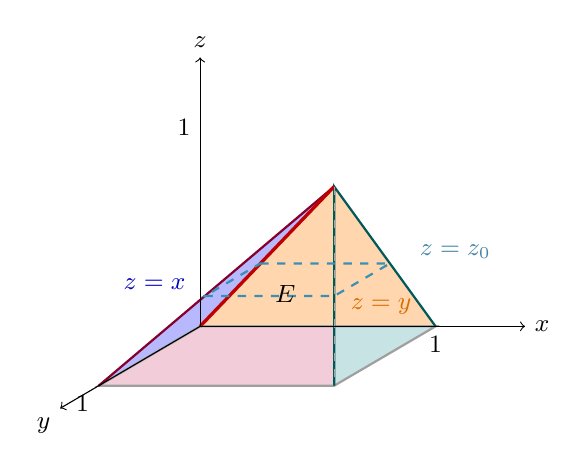
\begin{tikzpicture}[
    x={(3.25cm,0cm)}, y={(-1.4cm,-.82cm)}, z={(0cm,2.75cm)},
    scale=.92, every node/.style={font=\small}]
    % Base cuadrada z=0.
    \fill[gray!14] (0,0,0) -- (1,0,0) -- (1,1,0) -- (0,1,0) -- cycle;

    % Caras verticales x=1 y y=1.
    \fill[teal!22] (1,0,0) -- (1,1,0) -- (1,1,1) -- cycle;
    \fill[purple!20] (0,1,0) -- (1,1,0) -- (1,1,1) -- cycle;

    % Los dos techos del sólido.
    \fill[orange!32] (0,0,0) -- (1,0,0) -- (1,1,1) -- cycle;
    \fill[blue!28] (0,0,0) -- (0,1,0) -- (1,1,1) -- cycle;

    % Aristas y cresta donde z=x=y.
    \draw[gray!75,thick] (0,0,0) -- (1,0,0) -- (1,1,0) -- (0,1,0) -- cycle;
    \draw[teal!70!black,thick] (1,0,0) -- (1,1,1) -- (1,1,0);
    \draw[purple!70!black,thick] (0,1,0) -- (1,1,1);
    \draw[red!75!black,very thick] (0,0,0) -- (1,1,1);
    \draw[dashed,gray!70] (1,1,1) -- (1,1,0);

    % Corte horizontal z=z_0; sus lados tienen longitud 1-z_0.
    \draw[cyan!70!black,dashed,thick]
        (.45,.45,.45) -- (1,.45,.45) -- (1,1,.45)
        -- (.45,1,.45) -- cycle;
    \node[cyan!60!black,right] at (1,.25,.45) {$z=z_0$};

    % Ejes y etiquetas.
    \draw[->] (0,0,0) -- (1.38,0,0) node[right] {$x$};
    \draw[->] (0,0,0) -- (0,1.38,0) node[below left] {$y$};
    \draw[->] (0,0,0) -- (0,0,1.35) node[above] {$z$};
    \node at (.62,.6,.34) {$E$};
    \node[orange!85!black,below right] at (.62,.05,.2) {$z=y$};
    \node[blue!75!black,left] at (.28,.7,.42) {$z=x$};
    \node[below] at (1,0,0) {$1$};
    \node[below left] at (0,1,0) {$1$};
    \node[left] at (0,0,1) {$1$};
\end{tikzpicture}
\hspace{.5cm}
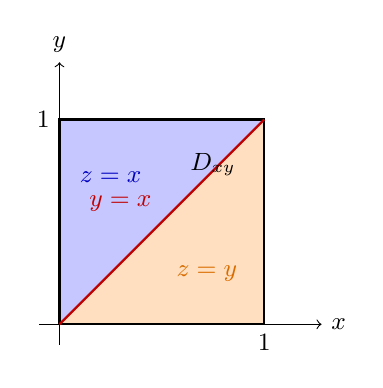
\begin{tikzpicture}[scale=2.6,every node/.style={font=\small}]
    \fill[orange!25] (0,0) -- (1,0) -- (1,1) -- cycle;
    \fill[blue!22] (0,0) -- (0,1) -- (1,1) -- cycle;
    \draw[->] (-.1,0) -- (1.28,0) node[right] {$x$};
    \draw[->] (0,-.1) -- (0,1.28) node[above] {$y$};
    \draw[thick] (0,0) rectangle (1,1);
    \draw[red!75!black,thick] (0,0) -- (1,1)
        node[midway,above left] {$y=x$};
    \node[orange!85!black] at (.72,.25) {$z=y$};
    \node[blue!75!black] at (.25,.72) {$z=x$};
    \node[below] at (1,0) {$1$};
    \node[left] at (0,1) {$1$};
    \node at (.75,.78) {$D_{xy}$};
\end{tikzpicture}
\end{center}
\endgroup

La cresta roja satisface $x=y=z$. Su proyección es la diagonal $y=x$, que separa las dos fórmulas del techo. El cuadrado punteado representa un corte a altura $z_0$: en él se cumple $z_0\leq x\leq1$ y $z_0\leq y\leq1$.
\end{samepage}

\begin{align*}
V&=\int_0^1\int_0^x\int_0^y1\,dz\,dy\,dx
+\int_0^1\int_x^1\int_0^x1\,dz\,dy\,dx\\
&=\int_0^1\left(\frac{x^2}{2}+x(1-x)\right)dx=\frac13.
\end{align*}
Si se deja $z$ para el final, las desigualdades se convierten en
\[
0\leq z\leq1,\qquad z\leq x\leq1,\qquad z\leq y\leq1.
\]
Cada corte horizontal es un cuadrado de lado $1-z$ y basta una sola integral:
\[
V=\int_0^1\int_z^1\int_z^1 1\,dy\,dx\,dz
=\int_0^1(1-z)^2\,dz=\frac13.
\]
Este ejemplo muestra por qué conviene comparar las proyecciones y los cortes antes de efectuar el cálculo.

\paragraph{Ejemplo 6.Un hueco}

Se considera el sólido entre dos esferas concéntricas,
\[
E=\{(x,y,z):1\leq x^2+y^2+z^2\leq4\}.
\]

\begin{samepage}
\begingroup
\shorthandoff{>}
\begin{center}
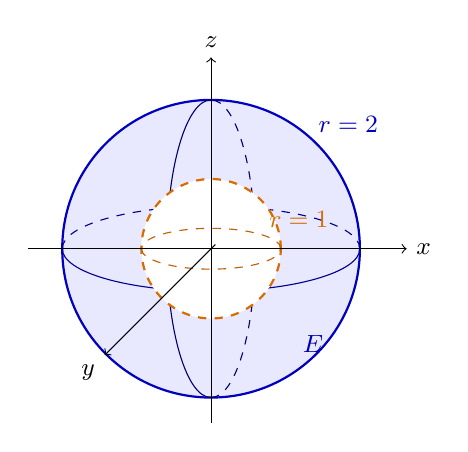
\begin{tikzpicture}[scale=1.08,every node/.style={font=\small}]
    % Vista espacial de las dos fronteras esféricas.
    \fill[blue!9] (0,0) circle (1.75);
    \draw[blue!75!black,thick] (0,0) circle (1.75);
    \draw[blue!55!black] (-1.75,0) arc[start angle=180,end angle=360,x radius=1.75,y radius=.5];
    \draw[blue!55!black,dashed] (1.75,0) arc[start angle=0,end angle=180,x radius=1.75,y radius=.5];
    \draw[blue!45!black,dashed] (0,-1.75) arc[start angle=-90,end angle=90,x radius=.52,y radius=1.75];
    \draw[blue!45!black] (0,1.75) arc[start angle=90,end angle=270,x radius=.52,y radius=1.75];

    \fill[white] (0,0) circle (.82);
    \draw[orange!85!black,thick,dashed] (0,0) circle (.82);
    \draw[orange!75!black,dashed] (-.82,0) arc[start angle=180,end angle=360,x radius=.82,y radius=.24];
    \draw[orange!75!black,dashed] (.82,0) arc[start angle=0,end angle=180,x radius=.82,y radius=.24];

    \draw[->] (-2.15,0) -- (2.3,0) node[right] {$x$};
    \draw[->] (0,-2.05) -- (0,2.25) node[above] {$z$};
    \draw[->] (.05,.05) -- (-1.25,-1.25) node[below left] {$y$};
    \node[blue!75!black,above right] at (1.15,1.25) {$r=2$};
    \node[orange!85!black,below right] at (.57,.55) {$r=1$};
    \node[blue!70!black] at (1.2,-1.12) {$E$};
\end{tikzpicture}
\hspace{.65cm}
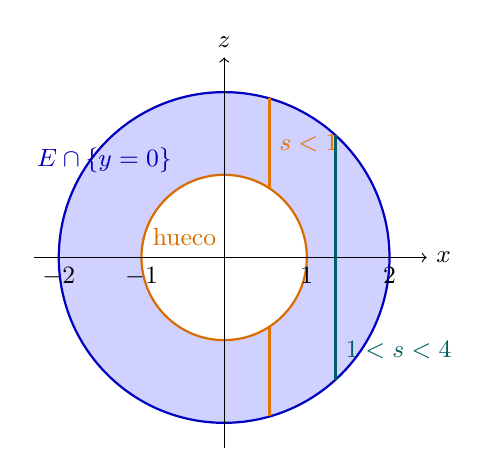
\begin{tikzpicture}[scale=1.05,every node/.style={font=\small}]
    % Corte por el plano y=0: una corona circular en el plano xz.
    \fill[blue!18,even odd rule] (0,0) circle (2) (0,0) circle (1);
    \draw[blue!75!black,thick] (0,0) circle (2);
    \draw[orange!85!black,thick] (0,0) circle (1);
    \draw[->] (-2.3,0) -- (2.45,0) node[right] {$x$};
    \draw[->] (0,-2.3) -- (0,2.42) node[above] {$z$};

    % Para |x|<1 aparecen dos intervalos separados por el hueco.
    \draw[orange!90!black,very thick] (.55,.835) -- (.55,1.923);
    \draw[orange!90!black,very thick] (.55,-1.923) -- (.55,-.835);
    \node[orange!90!black,right] at (.55,1.38) {$s<1$};

    % Para 1<|x|<2 aparece un solo intervalo vertical.
    \draw[teal!75!black,very thick] (1.35,-1.476) -- (1.35,1.476);
    \node[teal!75!black,right] at (1.35,-1.12) {$1<s<4$};

    \node[blue!70!black] at (-1.45,1.18) {$E\cap\{y=0\}$};
    \node[orange!85!black] at (-.48,.25) {hueco};
    \node[below] at (2,0) {$2$};
    \node[below] at (1,0) {$1$};
    \node[below] at (-1,0) {$-1$};
    \node[below] at (-2,0) {$-2$};
\end{tikzpicture}
\end{center}
\endgroup

La esfera naranja delimita el hueco y la esfera azul delimita el exterior del sólido. En el corte $y=0$, la recta naranja con $|x|<1$ atraviesa $E$ en dos segmentos separados. La recta verde azulada con $1<|x|<2$ lo atraviesa en un solo segmento.
\end{samepage}

Para abreviar, se escribe $s=x^2+y^2$, $h_2=\sqrt{4-s}$ y, cuando $s\leq1$, $h_1=\sqrt{1-s}$. Si $s<1$, la recta vertical corta el sólido en dos intervalos:
\[
-h_2\leq z\leq-h_1,\qquad h_1\leq z\leq h_2.
\]
Si $1\leq s\leq4$, hay un solo intervalo $-h_2\leq z\leq h_2$. Sean $D_1=\{(x,y):s\leq1\}$ y $D_2=\{(x,y):1\leq s\leq4\}$. Entonces
\begin{align*}
\iiint_E f\,dV
&=\iint_{D_1}\left(\int_{-h_2}^{-h_1} f(x,y,z)\,dz
+\int_{h_1}^{h_2} f(x,y,z)\,dz\right)dA\\
&\quad+\iint_{D_2}\left(\int_{-h_2}^{h_2}f(x,y,z)\,dz\right)dA.
\end{align*}
Las fronteras compartidas no afectan el valor. En particular, usar $-h_2\leq z\leq h_2$ sobre todo el disco de radio $2$ incluiría la esfera interior que se ha retirado.

Para el volumen resulta más breve restar las integrales de las dos bolas. Sus cortes horizontales dan
\begin{align*}
V&=\int_{-2}^{2}\pi(4-z^2)\,dz
-\int_{-1}^{1}\pi(1-z^2)\,dz\\
&=\frac{32\pi}{3}-\frac{4\pi}{3}=\frac{28\pi}{3}.
\end{align*}
Esta resta también sirve para un integrando definido y continuo en toda la bola exterior. Si $f$ solo está definida en $E$, la expresión por segmentos evita requerir valores dentro del hueco.

\subsection{Aplicaciones de la integral triple}

Una integral triple permite acumular una cantidad distribuida en un sólido. Si cada elemento de volumen $dV$ aporta una cantidad $f(x,y,z)\,dV$, la contribución total se obtiene mediante $\iiint_E f\,dV$. La elección del integrando depende de la magnitud física o geométrica que se desea calcular.

\subsubsection{Cálculo de volúmenes}

El volumen de un sólido medible y acotado $E$ se obtiene integrando la función constante $1$:
\[
V(E)=\iiint_E 1\,dV.
\]
Los límites describen el sólido y el integrando cuenta una unidad de volumen por cada elemento $dV$. Cuando $E$ queda entre $z=u(x,y)$ y $z=v(x,y)$ sobre una proyección $D_{xy}$, se tiene
\[
V(E)=\iint_{D_{xy}}\bigl(v(x,y)-u(x,y)\bigr)\,dA.
\]
Esta igualdad se obtiene al efectuar primero la integral respecto de $z$.

\paragraph{Ejemplo de volumen.} Se considera el sólido limitado inferiormente por el paraboloide $z=x^2+y^2$ y superiormente por el plano $z=4$. Ambas superficies se intersectan en $x^2+y^2=4$, por lo que la proyección sobre $xy$ es el disco de radio $2$.

\begingroup
\shorthandoff{>}
\begin{center}
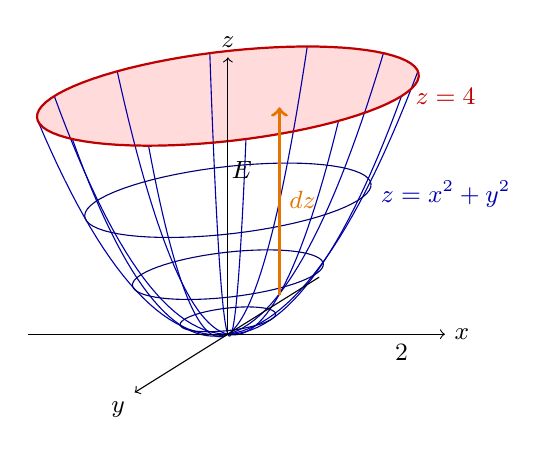
\begin{tikzpicture}[
    x={(1.05cm,0cm)}, y={(-.48cm,-.3cm)}, z={(0cm,.72cm)},
    scale=1.05,every node/.style={font=\small}]
    % Plano superior y superficie parabólica.
    \fill[red!14] plot[domain=0:360,samples=80]
        ({2*cos(\x)},{2*sin(\x)},4) -- cycle;
    \foreach \ang in {0,30,...,330} {
        \draw[blue!65!black] plot[domain=0:2,samples=30]
            ({\x*cos(\ang)},{\x*sin(\ang)},{\x*\x});
    }
    \foreach \rad in {.5,1,1.5} {
        \draw[blue!45!black] plot[domain=0:360,samples=70]
            ({\rad*cos(\x)},{\rad*sin(\x)},{\rad*\rad});
    }
    \draw[red!75!black,thick] plot[domain=0:360,samples=80]
        ({2*cos(\x)},{2*sin(\x)},4);

    % Segmento vertical que recorre el volumen.
    \draw[orange!90!black,very thick,->] (.8,.45,{.8*.8+.45*.45}) -- (.8,.45,4);
    \node[orange!90!black,right] at (.8,.45,2.45) {$dz$};

    \draw[->] (-2.3,0,0) -- (2.5,0,0) node[right] {$x$};
    \draw[->] (0,-2.3,0) -- (0,2.35,0) node[below left] {$y$};
    \draw[->] (0,0,0) -- (0,0,4.65) node[above] {$z$};
    \node[red!75!black,right] at (2.05,0,4) {$z=4$};
    \node[blue!70!black,right] at (1.65,0,2.35) {$z=x^2+y^2$};
    \node at (.25,.2,2.85) {$E$};
    \node[below] at (2,0,0) {$2$};
\end{tikzpicture}
\end{center}
\endgroup

En coordenadas cartesianas, el volumen se formula como
\[
V=\int_{-2}^{2}\int_{-\sqrt{4-x^2}}^{\sqrt{4-x^2}}
\int_{x^2+y^2}^{4}1\,dz\,dy\,dx.
\]
Después de integrar respecto de $z$, la simetría circular permite usar coordenadas polares en la proyección. Como $dA=r\,dr\,d\theta$,
\begin{align*}
V&=\int_0^{2\pi}\int_0^2(4-r^2)r\,dr\,d\theta\\
&=2\pi\left[2r^2-\frac{r^4}{4}\right]_0^2=8\pi.
\end{align*}

\subsubsection{Densidades: masa y carga eléctrica}

Una densidad volumétrica indica cuánta cantidad se concentra por unidad de volumen cerca de cada punto. Si $\rho_m(x,y,z)\geq0$ es una densidad de masa, entonces
\[
dm=\rho_m(x,y,z)\,dV,
\qquad
m=\iiint_E\rho_m(x,y,z)\,dV.
\]
La densidad media de un sólido de volumen positivo es
\[
\rho_{\mathrm{med}}=\frac{m}{V(E)}.
\]
Si $\rho_e(x,y,z)$ representa densidad volumétrica de carga eléctrica, la carga total es
\[
dQ=\rho_e(x,y,z)\,dV,
\qquad
Q=\iiint_E\rho_e(x,y,z)\,dV.
\]
A diferencia de la densidad de masa, $\rho_e$ puede ser positiva o negativa. Por ello, regiones con cargas de signos opuestos pueden cancelarse al calcular $Q$.

\paragraph{Ejemplo de masa.} El tetraedro
\[
E=\{(x,y,z):x\geq0,\ y\geq0,\ z\geq0,\ x+y+z\leq1\}
\]
tiene densidad $\rho_m(x,y,z)=\rho_0(1+z)$, donde $\rho_0>0$. La densidad aumenta con la altura.

\begingroup
\shorthandoff{>}
\begin{center}
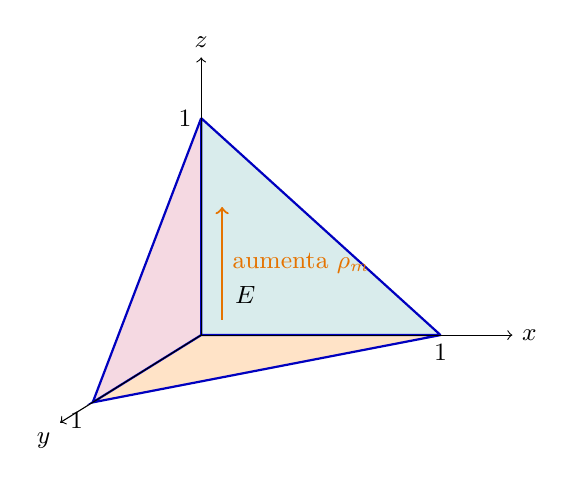
\begin{tikzpicture}[
    x={(3.2cm,0cm)}, y={(-1.45cm,-.9cm)}, z={(0cm,2.9cm)},
    scale=.95,every node/.style={font=\small}]
    \fill[blue!16] (0,0,0) -- (1,0,0) -- (0,1,0) -- cycle;
    \fill[orange!22] (1,0,0) -- (0,1,0) -- (0,0,1) -- cycle;
    \fill[purple!15] (0,0,0) -- (0,1,0) -- (0,0,1) -- cycle;
    \fill[teal!15] (0,0,0) -- (1,0,0) -- (0,0,1) -- cycle;
    \draw[blue!75!black,thick]
        (0,0,0) -- (1,0,0) -- (0,1,0) -- cycle
        (0,0,0) -- (0,0,1)
        (1,0,0) -- (0,0,1)
        (0,1,0) -- (0,0,1);
    \draw[->,orange!90!black,thick] (.16,.16,.12) -- (.16,.16,.64)
        node[midway,right] {aumenta $\rho_m$};
    \draw[->] (0,0,0) -- (1.3,0,0) node[right] {$x$};
    \draw[->] (0,0,0) -- (0,1.3,0) node[below left] {$y$};
    \draw[->] (0,0,0) -- (0,0,1.28) node[above] {$z$};
    \node at (.32,.3,.28) {$E$};
    \node[below] at (1,0,0) {$1$};
    \node[below left] at (0,1,0) {$1$};
    \node[left] at (0,0,1) {$1$};
\end{tikzpicture}
\end{center}
\endgroup

Su masa se calcula mediante
\begin{align*}
m
&=\rho_0\int_0^1\int_0^{1-x}\int_0^{1-x-y}(1+z)\,dz\,dy\,dx\\
&=\rho_0\int_0^1\int_0^{1-x}
\left[(1-x-y)+\frac{(1-x-y)^2}{2}\right]dy\,dx
=\frac{5\rho_0}{24}.
\end{align*}
El término constante aporta $\rho_0/6$ y el término que depende de $z$ aporta $\rho_0/24$. La mayor densidad cerca del vértice superior incrementa la masa respecto del tetraedro homogéneo de densidad $\rho_0$.

\paragraph{Ejemplo de carga eléctrica.} Se considera la caja
\[
E=[-1,1]\times[0,1]\times[0,1]
\]
con densidad de carga $\rho_e(x,y,z)=\rho_0x$, donde $\rho_0>0$ es una constante con unidades compatibles. La mitad con $x<0$ tiene carga negativa y la mitad con $x>0$ tiene carga positiva.

\begingroup
\shorthandoff{>}
\begin{center}
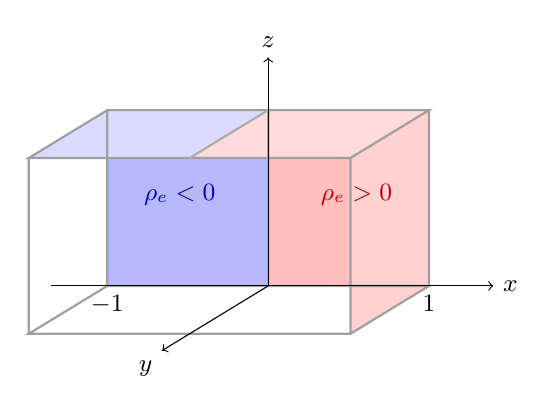
\begin{tikzpicture}[
    x={(2.15cm,0cm)}, y={(-1.05cm,-.64cm)}, z={(0cm,2.35cm)},
    scale=.95,every node/.style={font=\small}]
    \fill[blue!28] (-1,0,0) -- (0,0,0) -- (0,0,1) -- (-1,0,1) -- cycle;
    \fill[red!25] (0,0,0) -- (1,0,0) -- (1,0,1) -- (0,0,1) -- cycle;
    \fill[blue!14] (-1,0,1) -- (0,0,1) -- (0,1,1) -- (-1,1,1) -- cycle;
    \fill[red!14] (0,0,1) -- (1,0,1) -- (1,1,1) -- (0,1,1) -- cycle;
    \fill[red!18] (1,0,0) -- (1,1,0) -- (1,1,1) -- (1,0,1) -- cycle;
    \draw[gray!75,thick]
        (-1,0,0) -- (1,0,0) -- (1,1,0) -- (-1,1,0) -- cycle
        (-1,0,1) -- (1,0,1) -- (1,1,1) -- (-1,1,1) -- cycle
        (-1,0,0) -- (-1,0,1)
        (1,0,0) -- (1,0,1)
        (1,1,0) -- (1,1,1)
        (-1,1,0) -- (-1,1,1);
    \draw[gray!65,thick] (0,0,0) -- (0,0,1) -- (0,1,1);
    \draw[->] (-1.35,0,0) -- (1.4,0,0) node[right] {$x$};
    \draw[->] (0,0,0) -- (0,1.35,0) node[below left] {$y$};
    \draw[->] (0,0,0) -- (0,0,1.3) node[above] {$z$};
    \node[blue!75!black] at (-.55,0,.52) {$\rho_e<0$};
    \node[red!75!black] at (.55,0,.52) {$\rho_e>0$};
    \node[below] at (-1,0,0) {$-1$};
    \node[below] at (1,0,0) {$1$};
\end{tikzpicture}
\end{center}
\endgroup

Las cargas de cada mitad son
\begin{align*}
Q_-&=\rho_0\int_{-1}^{0}\int_0^1\int_0^1x\,dz\,dy\,dx=-\frac{\rho_0}{2},\\
Q_+&=\rho_0\int_{0}^{1}\int_0^1\int_0^1x\,dz\,dy\,dx=\frac{\rho_0}{2}.
\end{align*}
En consecuencia,
\[
Q=Q_-+Q_+=0.
\]
La carga total nula no significa que la caja carezca de carga: las cantidades positiva y negativa tienen la misma magnitud y se cancelan.

\subsubsection{Momentos de inercia}

Sea $\rho(x,y,z)\geq0$ la densidad volumétrica de un sólido $E$. El momento de inercia respecto de un eje suma cada elemento de masa multiplicado por el cuadrado de su distancia al eje. Respecto de los tres ejes coordenados,
\begin{align*}
I_x&=\iiint_E(y^2+z^2)\rho(x,y,z)\,dV,\\
I_y&=\iiint_E(x^2+z^2)\rho(x,y,z)\,dV,\\
I_z&=\iiint_E(x^2+y^2)\rho(x,y,z)\,dV.
\end{align*}
Por ejemplo, la distancia al eje $z$ es $\sqrt{x^2+y^2}$, lo que explica el factor $x^2+y^2$ en $I_z$. Si la densidad se mide en masa por unidad de volumen, un momento de inercia tiene unidades de masa multiplicada por longitud al cuadrado.

\paragraph{Ejemplo de momentos de inercia.} Se considera el prisma rectangular homogéneo
\[
E=[-a,a]\times[-b,b]\times[-c,c],
\qquad a,b,c>0,
\]
con densidad constante $\rho_0$. Sus dimensiones son $2a$, $2b$ y $2c$, y su centro geométrico se encuentra en el origen.

\begingroup
\shorthandoff{>}
\begin{center}
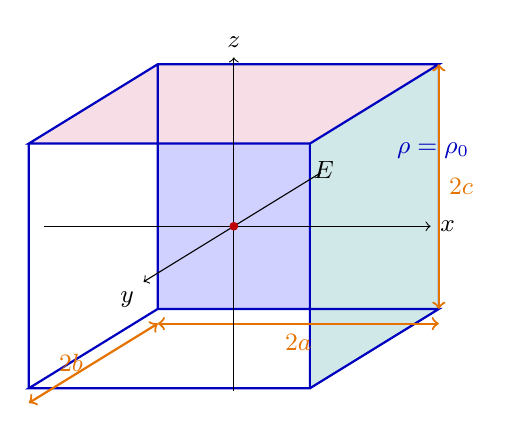
\begin{tikzpicture}[
    x={(1.7cm,0cm)}, y={(-.78cm,-.48cm)}, z={(0cm,1.48cm)},
    scale=1.05,every node/.style={font=\small}]
    \fill[blue!18] (-1,-1,-1) -- (1,-1,-1) -- (1,-1,1) -- (-1,-1,1) -- cycle;
    \fill[teal!18] (1,-1,-1) -- (1,1,-1) -- (1,1,1) -- (1,-1,1) -- cycle;
    \fill[purple!13] (-1,-1,1) -- (1,-1,1) -- (1,1,1) -- (-1,1,1) -- cycle;
    \draw[blue!75!black,thick]
        (-1,-1,-1) -- (1,-1,-1) -- (1,1,-1) -- (-1,1,-1) -- cycle
        (-1,-1,1) -- (1,-1,1) -- (1,1,1) -- (-1,1,1) -- cycle
        (-1,-1,-1) -- (-1,-1,1)
        (1,-1,-1) -- (1,-1,1)
        (1,1,-1) -- (1,1,1)
        (-1,1,-1) -- (-1,1,1);

    \draw[<->,orange!90!black,thick] (-1,-1,-1.12) -- (1,-1,-1.12)
        node[midway,below] {$2a$};
    \draw[<->,orange!90!black,thick] (-1,-1,-1.12) -- (-1,1,-1.12)
        node[midway,left] {$2b$};
    \draw[<->,orange!90!black,thick] (1,-1,-1) -- (1,-1,1)
        node[midway,right] {$2c$};
    \draw[->] (-1.35,0,0) -- (1.4,0,0) node[right] {$x$};
    \draw[->] (0,-1.35,0) -- (0,1.4,0) node[below left] {$y$};
    \draw[->] (0,0,-1.35) -- (0,0,1.38) node[above] {$z$};
    \fill[red!75!black] (0,0,0) circle (1.5pt);
    \node at (.48,-.35,.35) {$E$};
    \node[blue!75!black,right] at (1,-.2,.55) {$\rho=\rho_0$};
\end{tikzpicture}
\end{center}
\endgroup

La masa del prisma es
\[
M=\rho_0(2a)(2b)(2c)=8abc\rho_0.
\]
Para el eje $x$, el cálculo se realiza únicamente con límites rectangulares:
\begin{align*}
I_x
&=\rho_0\int_{-a}^{a}\int_{-b}^{b}\int_{-c}^{c}
(y^2+z^2)\,dz\,dy\,dx\\
&=\rho_0(2a)\left[
\left(\frac{2b^3}{3}\right)(2c)
+(2b)\left(\frac{2c^3}{3}\right)\right]\\
&=\frac{M}{3}(b^2+c^2).
\end{align*}
Al permutar las variables se obtienen los otros dos momentos:
\[
I_y=\frac{M}{3}(a^2+c^2),
\qquad
I_z=\frac{M}{3}(a^2+b^2).
\]

\subsubsection{Centro de masa}

La masa total y los primeros momentos de un sólido con densidad $\rho$ son
\begin{align*}
m&=\iiint_E\rho\,dV,\\
M_{yz}&=\iiint_E x\rho\,dV,\qquad
M_{xz}=\iiint_E y\rho\,dV,\qquad
M_{xy}=\iiint_E z\rho\,dV.
\end{align*}
El subíndice indica el plano respecto del cual se calcula el momento. Si $m>0$, el centro de masa es
\[
(\bar x,\bar y,\bar z)
=\left(\frac{M_{yz}}m,\frac{M_{xz}}m,\frac{M_{xy}}m\right).
\]
Cada coordenada es un promedio ponderado por la densidad. Por ello, el centro de masa se desplaza hacia las regiones donde $\rho$ es mayor.

\paragraph{Ejemplo de centro de masa.} El cubo unitario $E=[0,1]^3$ tiene densidad
\[
\rho(x,y,z)=1+x.
\]
La densidad aumenta en la dirección positiva del eje $x$.

\begingroup
\shorthandoff{>}
\begin{center}
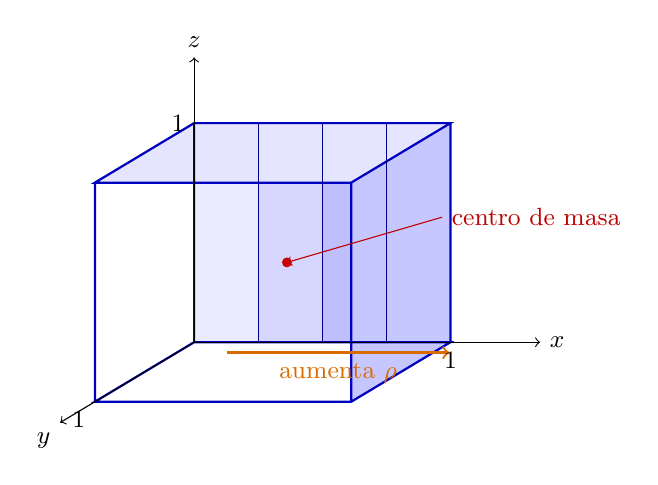
\begin{tikzpicture}[
    x={(3.1cm,0cm)}, y={(-1.2cm,-.72cm)}, z={(0cm,2.65cm)},
    scale=1.05,every node/.style={font=\small}]
    % Gradiente de densidad sobre la cara frontal.
    \fill[blue!8] (0,0,0) -- (.25,0,0) -- (.25,0,1) -- (0,0,1) -- cycle;
    \fill[blue!16] (.25,0,0) -- (.5,0,0) -- (.5,0,1) -- (.25,0,1) -- cycle;
    \fill[blue!25] (.5,0,0) -- (.75,0,0) -- (.75,0,1) -- (.5,0,1) -- cycle;
    \fill[blue!36] (.75,0,0) -- (1,0,0) -- (1,0,1) -- (.75,0,1) -- cycle;
    \fill[blue!22] (1,0,0) -- (1,1,0) -- (1,1,1) -- (1,0,1) -- cycle;
    \fill[blue!10] (0,0,1) -- (1,0,1) -- (1,1,1) -- (0,1,1) -- cycle;

    \draw[blue!75!black,thick]
        (0,0,0) -- (1,0,0) -- (1,1,0) -- (0,1,0) -- cycle
        (0,0,1) -- (1,0,1) -- (1,1,1) -- (0,1,1) -- cycle
        (0,0,0) -- (0,0,1)
        (1,0,0) -- (1,0,1)
        (1,1,0) -- (1,1,1)
        (0,1,0) -- (0,1,1);
    \foreach \t in {.25,.5,.75} {
        \draw[blue!55!black] (\t,0,0) -- (\t,0,1);
    }

    \fill[red!80!black] (.5556,.5,.5) circle (1.7pt);
    \draw[->,red!75!black] (1.18,.55,.72) node[right] {centro de masa}
        -- (.5556,.5,.5);
    \draw[->,orange!85!black,thick] (.08,-.12,-.08) -- (.95,-.12,-.08)
        node[midway,below] {aumenta $\rho$};
    \draw[->] (0,0,0) -- (1.35,0,0) node[right] {$x$};
    \draw[->] (0,0,0) -- (0,1.35,0) node[below left] {$y$};
    \draw[->] (0,0,0) -- (0,0,1.3) node[above] {$z$};
    \node[below] at (1,0,0) {$1$};
    \node[below left] at (0,1,0) {$1$};
    \node[left] at (0,0,1) {$1$};
\end{tikzpicture}
\end{center}
\endgroup

La masa y los primeros momentos son
\begin{align*}
m&=\int_0^1\int_0^1\int_0^1(1+x)\,dz\,dy\,dx=\frac32,\\
M_{yz}&=\int_0^1\int_0^1\int_0^1x(1+x)\,dz\,dy\,dx=\frac56,\\
M_{xz}&=\int_0^1\int_0^1\int_0^1y(1+x)\,dz\,dy\,dx=\frac34,\\
M_{xy}&=\int_0^1\int_0^1\int_0^1z(1+x)\,dz\,dy\,dx=\frac34.
\end{align*}
Por tanto,
\[
(\bar x,\bar y,\bar z)
=\left(\frac59,\frac12,\frac12\right).
\]
Las coordenadas $\bar y$ y $\bar z$ conservan el valor $1/2$ debido a la simetría de la densidad en esas direcciones. En cambio, $\bar x=5/9>1/2$ porque la densidad aumenta con $x$.

\subsection{Ejercicios}
\begin{enumerate}
    \item Evalúe
\[
\int_0^1\int_0^2\int_{-1}^{1}(x+2y-z)\,dz\,dy\,dx.
\]

    \item Evalúe
\[
\iiint_B x^2yz\,dV,
\qquad
B=[0,2]\times[1,3]\times[-1,1].
\]
Use el teorema de Fubini para comprobar el resultado.

    \item Evalúe
\[
\int_0^1\int_0^{1-x}\int_0^{1-x-y}(x+y+z)\,dz\,dy\,dx.
\]

    \item Evalúe $\iiint_E(x+z)\,dV$, donde
\[
E=\{(x,y,z):0\leq x\leq1,\ x\leq y\leq1,\ 0\leq z\leq y\}.
\]

    \item Evalúe la integral triple
\[
\int_0^1\int_0^{1-x}\int_{x+y}^{2-x-y}(x+y+z)\,dz\,dy\,dx.
\]
Grafique la región de integración.

    \item La figura muestra un sólido del primer octante limitado por el plano $x=0$, el cilindro parabólico $y=\sqrt{x}$, el plano $z=0$ y el plano inclinado $z=1-y$. Escriba $\iiint_E f(x,y,z)\,dV$ en los órdenes $dx\,dz\,dy$ y $dz\,dx\,dy$.

\begingroup
\shorthandoff{>}
\begin{center}
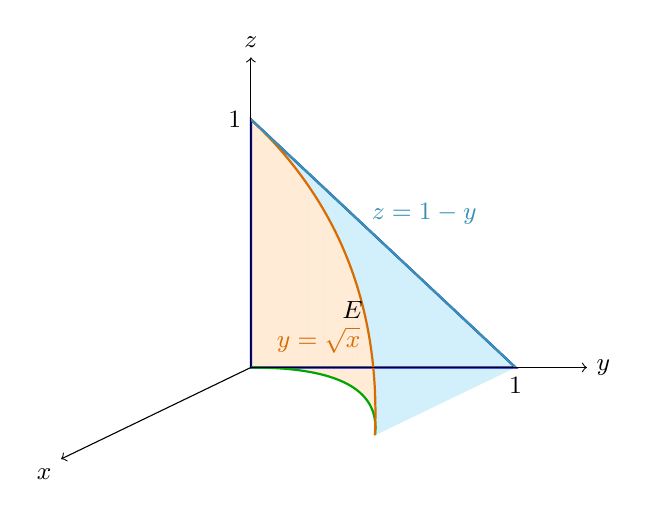
\begin{tikzpicture}[
    x={(-1.7cm,-.82cm)},y={(3.2cm,0cm)},z={(0cm,3cm)},
    scale=1.05,every node/.style={font=\small}]
    \fill[blue!11] (0,0,0) -- (0,1,0) -- (0,0,1) -- cycle;
    \fill[green!13] plot[domain=0:1,samples=35] ({\x*\x},{\x},0)
        -- (0,1,0) -- (0,0,0) -- cycle;
    \foreach \i in {0,...,11} {
        \pgfmathsetmacro{\ya}{\i/12}
        \pgfmathsetmacro{\yb}{(\i+1)/12}
        \fill[cyan!18]
            (0,\ya,{1-\ya}) -- ({\ya*\ya},\ya,{1-\ya}) --
            ({\yb*\yb},\yb,{1-\yb}) -- (0,\yb,{1-\yb}) -- cycle;
        \fill[orange!16]
            ({\ya*\ya},\ya,0) -- ({\yb*\yb},\yb,0) --
            ({\yb*\yb},\yb,{1-\yb}) -- ({\ya*\ya},\ya,{1-\ya}) -- cycle;
    }
    \draw[blue!75!black,thick] (0,0,0) -- (0,1,0) -- (0,0,1) -- cycle;
    \draw[green!65!black,thick]
        plot[domain=0:1,samples=45] ({\x*\x},{\x},0);
    \draw[orange!85!black,thick]
        plot[domain=0:1,samples=45] ({\x*\x},{\x},{1-\x});
    \draw[cyan!70!black,thick] (0,0,1) -- (0,1,0);
    \draw[->] (0,0,0) -- (1.35,0,0) node[below left] {$x$};
    \draw[->] (0,0,0) -- (0,1.27,0) node[right] {$y$};
    \draw[->] (0,0,0) -- (0,0,1.25) node[above] {$z$};
    \node[left] at (0,0,1) {$1$};
    \node[below] at (0,1,0) {$1$};
    \node[orange!85!black,left] at (.62,.78,.28) {$y=\sqrt{x}$};
    \node[cyan!70!black,right] at (0,.42,.62) {$z=1-y$};
    \node at (.18,.48,.28) {$E$};
\end{tikzpicture}
\end{center}
\endgroup

    \item La figura representa un sólido del primer octante limitado por el plano vertical $y=1-x$ y la superficie $z=1-x^2$. Formule $\iiint_E f\,dV$ en los órdenes $dz\,dy\,dx$ y $dy\,dx\,dz$.

\begingroup
\shorthandoff{>}
\begin{center}
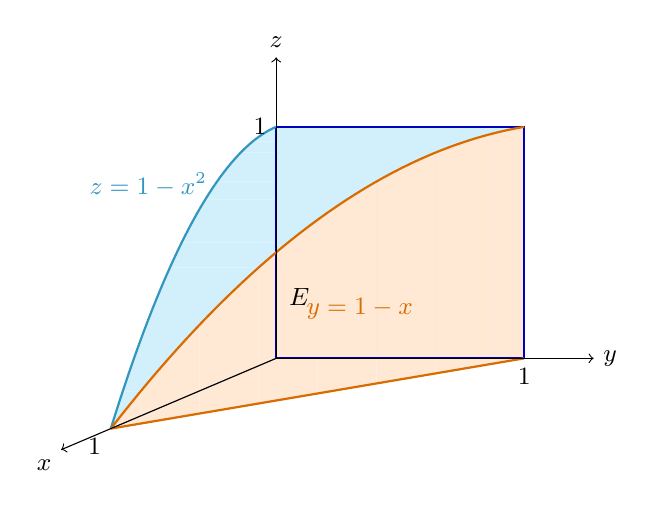
\begin{tikzpicture}[
    x={(-2cm,-.85cm)},y={(3cm,0cm)},z={(0cm,2.8cm)},
    scale=1.05,every node/.style={font=\small}]
    \fill[blue!10] (0,0,0) -- (0,1,0) -- (0,1,1) -- (0,0,1) -- cycle;
    \foreach \i in {0,...,13} {
        \pgfmathsetmacro{\xa}{\i/14}
        \pgfmathsetmacro{\xb}{(\i+1)/14}
        \fill[cyan!18]
            (\xa,0,{1-\xa*\xa}) -- (\xa,{1-\xa},{1-\xa*\xa}) --
            (\xb,{1-\xb},{1-\xb*\xb}) -- (\xb,0,{1-\xb*\xb}) -- cycle;
        \fill[orange!17]
            (\xa,{1-\xa},0) -- (\xb,{1-\xb},0) --
            (\xb,{1-\xb},{1-\xb*\xb}) --
            (\xa,{1-\xa},{1-\xa*\xa}) -- cycle;
    }
    \draw[blue!75!black,thick]
        (0,0,0) -- (0,1,0) -- (0,1,1) -- (0,0,1) -- cycle;
    \draw[cyan!75!black,thick]
        plot[domain=0:1,samples=45] (\x,0,{1-\x*\x});
    \draw[orange!85!black,thick]
        plot[domain=0:1,samples=45] (\x,{1-\x},{1-\x*\x});
    \draw[orange!85!black,thick] (0,1,0) -- (1,0,0);
    \draw[gray!65] (0,0,0) -- (1,0,0);
    \draw[->] (0,0,0) -- (1.3,0,0) node[below left] {$x$};
    \draw[->] (0,0,0) -- (0,1.28,0) node[right] {$y$};
    \draw[->] (0,0,0) -- (0,0,1.3) node[above] {$z$};
    \node[below left] at (1,0,0) {$1$};
    \node[below] at (0,1,0) {$1$};
    \node[left] at (0,0,1) {$1$};
    \node[cyan!75!black,left] at (.36,0,.86) {$z=1-x^2$};
    \node[orange!85!black,right] at (.55,.45,.38) {$y=1-x$};
    \node at (.28,.28,.35) {$E$};
\end{tikzpicture}
\end{center}
\endgroup

    \item La figura muestra un sólido del primer octante limitado por el cilindro parabólico $x=1-y^2$ y el plano $z=1-y$. Escriba $\iiint_E f\,dV$ en los órdenes $dx\,dz\,dy$ y $dz\,dy\,dx$.

\begingroup
\shorthandoff{>}
\begin{center}
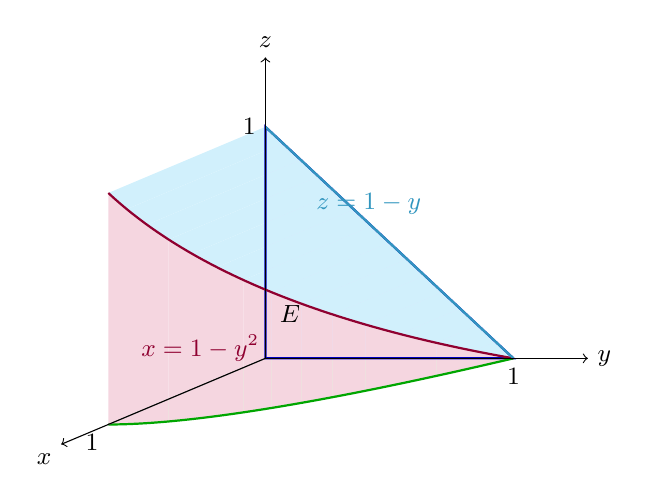
\begin{tikzpicture}[
    x={(-1.9cm,-.8cm)},y={(3cm,0cm)},z={(0cm,2.8cm)},
    scale=1.05,every node/.style={font=\small}]
    \fill[blue!10] (0,0,0) -- (0,1,0) -- (0,0,1) -- cycle;
    \fill[green!13] (0,0,0) -- (1,0,0) --
        plot[domain=0:1,samples=40] ({1-\x*\x},{\x},0) -- cycle;
    \foreach \i in {0,...,13} {
        \pgfmathsetmacro{\ya}{\i/14}
        \pgfmathsetmacro{\yb}{(\i+1)/14}
        \fill[cyan!18]
            (0,\ya,{1-\ya}) -- ({1-\ya*\ya},\ya,{1-\ya}) --
            ({1-\yb*\yb},\yb,{1-\yb}) -- (0,\yb,{1-\yb}) -- cycle;
        \fill[purple!16]
            ({1-\ya*\ya},\ya,0) -- ({1-\yb*\yb},\yb,0) --
            ({1-\yb*\yb},\yb,{1-\yb}) --
            ({1-\ya*\ya},\ya,{1-\ya}) -- cycle;
    }
    \draw[blue!75!black,thick] (0,0,0) -- (0,1,0) -- (0,0,1) -- cycle;
    \draw[green!65!black,thick]
        plot[domain=0:1,samples=45] ({1-\x*\x},{\x},0);
    \draw[purple!75!black,thick]
        plot[domain=0:1,samples=45] ({1-\x*\x},{\x},{1-\x});
    \draw[cyan!75!black,thick] (0,0,1) -- (0,1,0);
    \draw[gray!65] (0,0,0) -- (1,0,0);
    \draw[->] (0,0,0) -- (1.3,0,0) node[below left] {$x$};
    \draw[->] (0,0,0) -- (0,1.3,0) node[right] {$y$};
    \draw[->] (0,0,0) -- (0,0,1.3) node[above] {$z$};
    \node[below left] at (1,0,0) {$1$};
    \node[below] at (0,1,0) {$1$};
    \node[left] at (0,0,1) {$1$};
    \node[purple!75!black,left] at (.72,.47,.25) {$x=1-y^2$};
    \node[cyan!75!black,right] at (.18,.28,.72) {$z=1-y$};
    \node at (.38,.34,.3) {$E$};
\end{tikzpicture}
\end{center}
\endgroup

    \item La figura representa el sólido del primer octante comprendido entre el plano $y=x$ y el cilindro parabólico $z=9-x^2$. Formule $\iiint_E f\,dV$ en los órdenes $dz\,dy\,dx$ y $dy\,dx\,dz$.

\begingroup
\shorthandoff{>}
\begin{center}
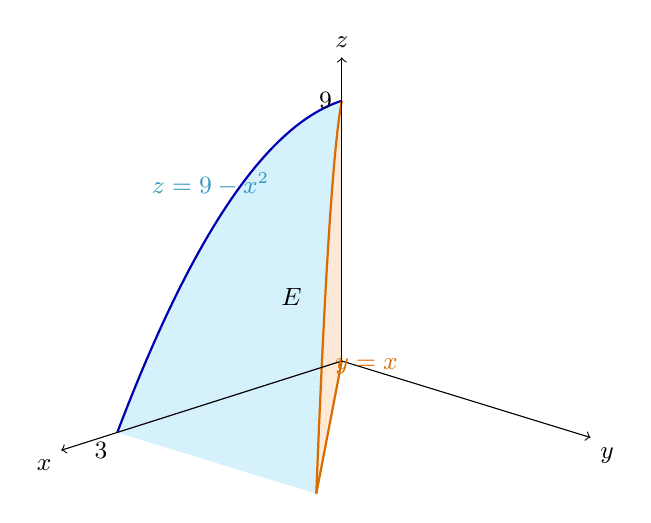
\begin{tikzpicture}[
    x={(-.88cm,-.28cm)},y={(.78cm,-.24cm)},z={(0cm,.34cm)},
    scale=1.08,every node/.style={font=\small}]
    \foreach \i in {0,...,17} {
        \pgfmathsetmacro{\xa}{3*\i/18}
        \pgfmathsetmacro{\xb}{3*(\i+1)/18}
        \fill[blue!11]
            (\xa,0,0) -- (\xb,0,0) -- (\xb,0,{9-\xb*\xb}) --
            (\xa,0,{9-\xa*\xa}) -- cycle;
        \fill[orange!17]
            (\xa,\xa,0) -- (\xb,\xb,0) --
            (\xb,\xb,{9-\xb*\xb}) -- (\xa,\xa,{9-\xa*\xa}) -- cycle;
        \fill[cyan!17]
            (\xa,0,{9-\xa*\xa}) -- (\xa,\xa,{9-\xa*\xa}) --
            (\xb,\xb,{9-\xb*\xb}) -- (\xb,0,{9-\xb*\xb}) -- cycle;
    }
    \draw[blue!70!black,thick]
        plot[domain=0:3,samples=50] (\x,0,{9-\x*\x});
    \draw[orange!85!black,thick]
        plot[domain=0:3,samples=50] (\x,\x,{9-\x*\x});
    \draw[orange!85!black,thick] (0,0,0) -- (3,3,0);
    \draw[gray!65] (0,0,0) -- (3,0,0);
    \draw[gray!65] (0,0,9) -- (0,0,0);
    \draw[->] (0,0,0) -- (3.75,0,0) node[below left] {$x$};
    \draw[->] (0,0,0) -- (0,3.75,0) node[below right] {$y$};
    \draw[->] (0,0,0) -- (0,0,10.5) node[above] {$z$};
    \node[below left] at (3,0,0) {$3$};
    \node[left] at (0,0,9) {$9$};
    \node[cyan!75!black,left] at (1.15,.35,7.3) {$z=9-x^2$};
    \node[orange!85!black,right] at (1.9,1.9,2.7) {$y=x$};
    \node at (1.25,.65,3.7) {$E$};
\end{tikzpicture}
\end{center}
\endgroup

    \item El sólido $E$ se encuentra en el primer octante y debajo del plano
\[
2x+3y+z=6.
\]
Dibuje $E$, identifique las intersecciones del plano con los ejes y formule una integral triple para su volumen en el orden $dz\,dy\,dx$.

    \item El sólido $E$ está limitado por $z=x^2$, $z=4$, $y=0$, $y=1$ y $x=0$, con $x\geq0$. Dibuje el sólido y formule $\iiint_E f(x,y,z)\,dV$.

    \item El sólido $E$ se encuentra dentro del cilindro $x^2+y^2=4$, encima del plano $z=0$ y debajo del paraboloide $z=x^2+y^2$. Dibuje el sólido y formule su volumen mediante una integral triple.

    \item El sólido $E$ satisface
\[
0\leq x\leq1,\qquad x^2\leq y\leq1,
\qquad 0\leq z\leq y.
\]
Dibuje las superficies que forman su frontera y formule $\iiint_E f\,dV$ con $y$ como variable interior.

    \item Dibuje el sólido descrito por
\[
\int_0^1\int_0^{1-x}\int_0^{1-x-y}
f(x,y,z)\,dz\,dy\,dx.
\]

    \item Dibuje el sólido descrito por
\[
\int_{-1}^{1}\int_{-\sqrt{1-x^2}}^{\sqrt{1-x^2}}
\int_0^{1-x^2-y^2} f(x,y,z)\,dz\,dy\,dx.
\]

    \item Dibuje el sólido cuyo volumen está dado por
\[
\int_0^1\int_0^x\int_0^y1\,dz\,dy\,dx
+\int_0^1\int_x^1\int_0^x1\,dz\,dy\,dx.
\]

    \item Considere la integral
\[
\int_0^1\int_0^{1-x}\int_0^{1-x-y}
f(x,y,z)\,dz\,dy\,dx.
\]
Describa geométricamente su región de integración y reescriba la integral en los otros cinco órdenes de integración.

    \item Sea
\[
E=\{(x,y,z):0\leq x\leq1,\ x^2\leq y\leq1,\ 0\leq z\leq y\}.
\]
La integral de $f$ sobre $E$ se expresa directamente en el orden $dz\,dy\,dx$. Reescríbala con $y$ como variable interior y $x$ como variable exterior.

    \item La región
\[
E=\{(x,y,z):0\leq x\leq y\leq z\leq1\}
\]
está representada por
\[
\int_0^1\int_y^1\int_0^y f(x,y,z)\,dx\,dz\,dy.
\]
    \item Evalúe
\[
\int_0^1\int_0^1\int_x^1 e^{z^2}\,dz\,dy\,dx.
\]

    \item El volumen bajo los dos techos $z=x$ y $z=y$ sobre el cuadrado $0\leq x,y\leq1$ está dado por
\[
\int_0^1\int_0^x\int_0^y1\,dz\,dy\,dx
+\int_0^1\int_x^1\int_0^x1\,dz\,dy\,dx.
\]
Reescriba la suma como una sola integral.
    \item Un sólido ocupa el tetraedro del primer octante limitado por el plano
\[
x+y+z=1
\]
y tiene densidad de masa $\rho(x,y,z)=\rho_0(1+z)$, donde $\rho_0>0$ es constante. Formule y calcule su masa. Determine también la densidad media
\[
\rho_{\mathrm{med}}=\frac{m}{V}.
\]

    \item El cubo $E=[0,1]^3$ tiene densidad de masa
\[
\rho(x,y,z)=1+x.
\]
Calcule la masa, los tres primeros momentos y el centro de masa.

    \item Un prisma rectangular está dado por
\[
E=[-a,a]\times[-b,b]\times[-c,c]
\]
y tiene masa total $M$. A partir de la densidad constante . Demuestre que sus momentos de inercia respecto de los ejes coordenados son
\[
I_x=\frac{M}{3}(b^2+c^2),\qquad
I_y=\frac{M}{3}(a^2+c^2),\qquad
I_z=\frac{M}{3}(a^2+b^2).
\]

    \item Una distribución de carga ocupa la caja
\[
E=[-1,1]\times[0,1]\times[0,1]
\]
y su densidad de carga es $\rho_e(x,y,z)=\rho_0x$, con $\rho_0>0$. Calcule por separado la carga positiva contenida en $x>0$, la carga negativa contenida en $x<0$ y la carga total.

\end{enumerate}